\documentclass[dvipdfmx]{jarticle}
\usepackage{graphicx}
\usepackage{url}
\usepackage[top=30truemm,bottom=30truemm,left=25truemm,right=25truemm]{geometry}
\usepackage{listings,jvlisting}

\lstset{
  basicstyle={\ttfamily},
  identifierstyle={\small},
  commentstyle={\smallitshape},
  keywordstyle={\small\bfseries},
  ndkeywordstyle={\small},
  stringstyle={\small\ttfamily},
  frame={tb},
  breaklines=true,
  columns=[l]{fullflexible},
  numbers=left,
  xrightmargin=0zw,
  xleftmargin=3zw,
  numberstyle={\scriptsize},
  stepnumber=1,
  numbersep=1zw,
  lineskip=-0.5ex
}

\begin{document}
\begin{titlepage}
    \begin{center}
        {\huge 情報科学演習C 課題3レポ―ト}
        \vspace{180pt}\\
        \begin{tabular}{rl}
            氏名 & 山久保孝亮\\
            所属 & 大阪大学基礎工学部情報科学科ソフトウェア科学コース\\
            メールアドレス & u327468b@ecs.osaka-u.ac.jp\\
            学籍番号 & 09B22084\\
            提出日 & \today\\
            担当教員 & 平井健士,中島悠太
        \end{tabular}
    \end{center}
\end{titlepage}
\section{課題3-1}
\subsection{アルゴリズム}
この課題の処理の流れは以下図1のフローチャートのとおりである.
\begin{figure}[h]
    \centering
    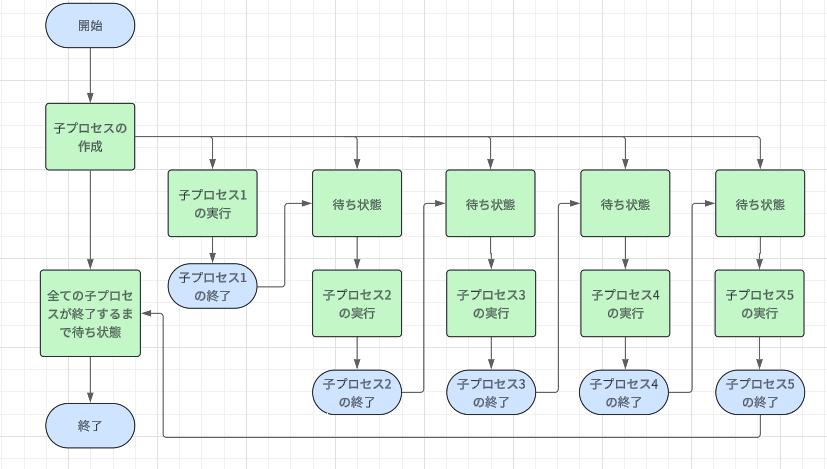
\includegraphics[width=12cm]{3-1hurotya.png}
    \caption{課題3-1の処理の流れ}
\end{figure}
\\
今回のfile-counterプログラムでは子プロセスを4つ作成し,それぞれの子プロセス内の処理を順番に一つずつ実行していく必要がある.
そのため,実行している子プロセス以外は待ち状態にしておき,実行が終了してから一つだけ待ち状態を開放して処理を実行するというアルゴリズムで今回の課題を実装した.フローチャートにおいて,子プロセスの終了から待ち状態へ伸びている矢印は
子プロセスが終わってから矢印の先の待ち状態が解放されるということを表している.今回の課題のクリティカルセクションは後述のcount1関数なので,この直前に待ち状態と解放を処理する関数を呼び出すようにした.
\subsection{実装方法}
ここではセマフォの処理について中心に記述する.以下は今回のプログラムにおける親プロセスの処理の流れである.
\begin{enumerate}
    \item セマフォセットの初期設定
    \item 子プロセスの作成
    \item 子プロセスがすべて終了するまで待つ
    \item セマフォの削除
\end{enumerate}
また,子プロセスの処理の流れは以下のようになる.
\begin{enumerate}
    \item lock()を呼び出す
    \item count1()を呼び出してファイルへの書き込み処理
    \item unlock()を呼び出す
    \item 子プロセスを終了
\end{enumerate}
以下でその詳細について記述する.
\begin{enumerate}
    \item まず,ftok()を使ってkeyを作成する.このとき,第一引数の"."は現在のディレクトリを表し,第二引数の"1"はプロジェクトを一意に識別する文字を指定している.\cite{1}次にsemget()を使ってセマフォセットを作成している.
    第一引数は作成したkey,第二引数はセマフォの数である4,第三引数はアクセス許可の定義として使用され,全てに読み込み,書き込み許可を与えるという設定である.\cite{2}最後にsemctl()を使って0番目のセマフォの値を1に設定する.
    第一引数はセマフォIDのsem\_idを,第二引数でセマフォ番号の0を,第三引数のSETVALはsemvalの値を第四引数で指定された値に設定する制御操作を指定するパラメータ値である.セマフォの初期値を1に設定する理由については子プロセス
    にて詳細を記述する.
    \item fork()を使って子プロセスを作成する.for文の中で呼び出すことによって子プロセスを複数作成する.fork()の返り値をpidに格納し,pidの値によって子プロセスを分岐させて親プロセスと子プロセスの処理内容を分ける.
    ここでは親プロセスについて記述するので,その後の親プロセスの処理について記述する.
    \item wait()を使って子プロセスの終了を待つ.引数には状況の情報値を格納する.2で作成したプロセスの数だけfor文でこれを繰り返すことですべてのプロセスが終了するまで待ち続けることができるようになる.\cite{3}
    \item 最後にセマフォをsemctl()を使って削除する.第三引数のIPC\_RMIDは第一引数によって指定されたセマフォIDをシステムから除去し,それに関連するセマフォセットを破棄する.\cite{2}
\end{enumerate}
次に,子プロセスの処理について記述する.
\begin{enumerate}
    \item 2においてpidの値が0のときは子プロセスであると判定できる.子プロセス内の処理がクリティカルセクションであるので,まずlock()を呼び出す.lock()では,semop()を使ってプロセスを停止している.第一引数はセマフォIDのsemid
    ,第二引数はsembuf構造体のポインタ,第三引数は第二引数の数を表す.sembuf構造体は3津のメンバが存在し,sem\_numはセマフォ番号,sem\_opはセマフォ操作,sem\_flagは操作フラグを表す.\cite{4}sem\_opは-1,それ以外は0に指定することによって
    セマフォ値がsem\_opの値を足した結果0以上にならない場合はプロセスを停止する.セマフォ値の初期値を1にしていたことによって,最初のプロセスは停止しないが,次のプロセスはセマフォ値が0でsem\_opを加算すると負の値になってしまうので
    停止する.
    \item セマフォに関係する処理はないので省略する.
    \item unlock()ではsemop()を使ってセマフォ値を変更し,子プロセスの待ち状態を一つ開放する.第二引数のsembuf構造体のsem\_opを1に,それ以外を0に設定することによって待っている一つの状態の子プロセスにおいて
    -1を加算してもセマフォ値が0以上になるので待ち状態ではなくなる.このようにして待ち状態のプロセスの開放を一つずつ行うことによってbクリティカルセクションに複数のプロセスが同時にアクセスできないようにしている.
    \item exit()を使って子プロセスを終了する.
\end{enumerate}
\subsection{実行結果}
\section{課題3-2-1}
\subsection{アルゴリズム}
この課題の処理の流れは以下図3のフローチャートのとおりである.
\begin{figure}[h]
    \centering
    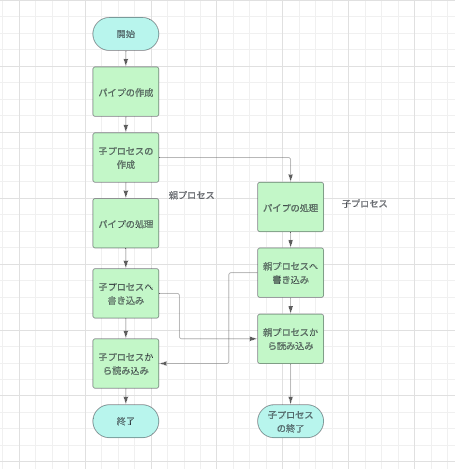
\includegraphics[width=8cm]{3-2hurotya.png}
    \caption{課題3-2の処理の流れ}
\end{figure}
\\
今回のtwo-way-pipeプログラムでは子プロセスを一つ作成し,子プロセスから親プロセスへ最初の引数の文字列を,親プロセスから子プロセスへ次の引数の文字列を送信する.
そして親プロセスは子プロセスから,子プロセスは親プロセスから送られてきた文字列を受け取り標準入力に表示させる.図の左側は親プロセス,右側は子プロセスの処理を表す.
双方向のパイプを実現するために,子プロセス用のパイプと親プロセス用のパイプの二つのパイプを作成して実装した.これは,パイプは安全のために書き込み側か読み込み側のどちらかをっクローズする必要があるため,
一つのパイプではどちらの機能も同時に使うことができないためである.
\subsection{実装方法}
パイプ部分を中心に実装方法を記述する.
\begin{enumerate}
    \item パイプの作成は,pipe()を使って行う.親プロセスから子プロセスへ送信したり,親プロセスが読み込むためのパイプとしてparenttochild,子プロセスから親プロセスへ送信したり,子プロセスが読み込むためのパイプとしてchildtoparent
    を定義した.
    \item fork()を使って子プロセスを一つ作成し,pidが0かどうかで親プロセスと子プロセスの処理を分離した.子プロセスではparenttochildの書き込み機能とchildtoparentの読み込み機能を使用しないので,これらをclose()しておく.
    そして第二引数の文字列をwrite()を使って送信しread()を使って親プロセスから送られてきた第一引数の文字列を受信して標準出力に出力する.また,親プロセスではparenttochildの読み込み機能とchildtoparentの書き込み機能を使用しないのでこれらをclose()しておく.
    そして第一引数の文字列をwrite()を使って送信しread()を使って子プロセスから送られてきた第二引数の文字列を受信して標準出力に出力する.
\end{enumerate}
\subsection{実行結果}
\section{課題3-2-2}
\subsection{アルゴリズム}
この課題の処理の流れは以下図5のフローチャートのとおりである.
\begin{figure}[h]
    \centering
    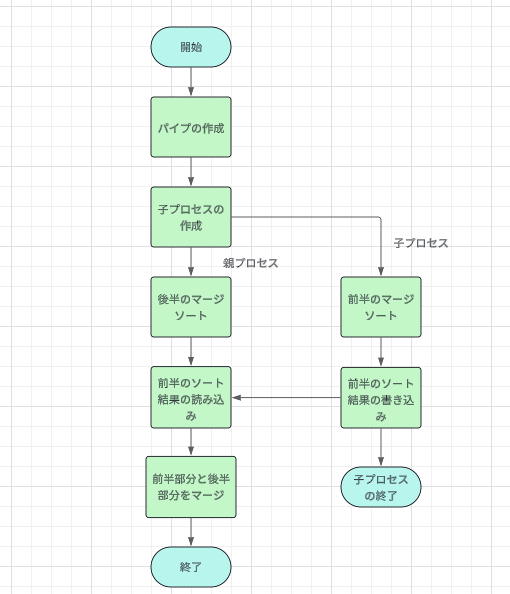
\includegraphics[width=8cm]{3-2-2hurotya.png}
    \caption{課題3-2の処理の流れ}
\end{figure}
\\
今回のmergesortプログラムでは子プロセスを一つ作成し,子プロセスでソート対象の配列の前半半分を,親プロセスでソート対象の配列の後半半分をソートしてからマージするというアルゴリズムで作成した.
図5の左側が親プロセス,右側が子プロセスに対応する.また,子プロセスのソート結果を親プロセスに伝えるためにパイプを使用した.これにより前半と後半のソートを並列に実行できるようになる.
\subsection{実装方法}
ここではマージソートのアルゴリズムについては言及せず,どのようにして並列化をしたかについて中心に記述する.関数mergesort中に図5のフローチャートの流れで並列化を実装したのでそれぞれの詳細について記述する.
\begin{enumerate}
    \item pipe()を使ってパイプfdを作成した.
    \item fork()を使って子プロセスを作成し,pidが0かどうかで親プロセスと子プロセスの処理を分離した.子プロセスではfdの読み込み機能は使用しないのでclose()しておく.引数には0と配列の要素の中央値を渡してmsort()呼び出す.
    これによってソート対象の配列の前半部分をマージソートすることができる.次にwrite()を呼び出して前半がソートされた配列を親プロセスに送信する.このときに引数に0と配列の要素の中央値を渡すことで配列全体ではなく前半部分のみを送ることができる.
    配列全体を送ってしまうと親プロセスでソートされた部分と競合してしまい,正しいソート結果ではなくなってしまう.
    \item 親プロセスではfdの書き込み機能は使用しないのでclose()しておく.親プロセスでは引数として配列の要素数の中央値と配列の要素数を渡してmsort()を呼び出す.これによってソート対象の配列の後半部分をマージソートすることができる.
    その後read()を使って子プロセスから送信された前半のソート結果を読み込む.このときに引数に配列の0と配列の要素数の中央値を渡すことで前半部分だけを読み込む.
    \item 最後に前半部分と後半部分をmergesort()を呼び出してソートする.
\end{enumerate}
\subsection{実行結果}
\section{課題3-3-1}
\subsection{アルゴリズム}

\subsection{実装方法}
\subsection{実行結果}
\section{課題3-3-2}
\subsection{アルゴリズム}
\subsection{実装方法}
\subsection{実行結果}
\begin{thebibliography}{99}
    \bibitem{1} \url{https://www.ibm.com/docs/ja/aix/7.3?topic=f-ftok-subroutine} 6/12アクセス
    \bibitem{2} \url{https://www.ibm.com/docs/ja/aix/7.3?topic=s-semget-subroutine} 6/12アクセス
    \bibitem{3} \url{https://www.ibm.com/docs/ja/zos/2.5.0?topic=functions-wait-wait-child-process-end} 6/12アクセス
    \bibitem{4} \url{https://www.c-lang.net/semop/index.html} 6/12アクセス
\end{thebibliography}
\end{document}